% this file is called up by thesis.tex
% content in this file will be fed into the main document

%: ----------------------- name of chapter  -------------------------
\chapter{Case Studies} % top level followed by section, subsection


Typing on a smartphone is made easier to the user by including auto-correct, but the same tool can not be used for authentication process. Therefore users are left with the task to hit every key accurately or repeat the task until they get it right. 

In this chapter we present the results from a survey made to determine, whether the proposed authentication method increases the user experience.


%: ----------------------- paths to graphics ------------------------

% change according to folder and file names
\ifpdf
    \graphicspath{{X/figures/PNG/}{X/figures/PDF/}{X/figures/}}
\else
    \graphicspath{{X/figures/EPS/}{X/figures/}}
\fi

%: ----------------------- contents from here ------------------------

%\input{4/File1}	
%\input{4/File}

\section{Validation}
In order to validate the hypothesis, the proposed solution is compared to the conventional ''input credentials'' method in terms of simplicity and user experience. A use case based on social media sign-in was developed. The application is primitive to only test the authentication process. 
	
In the first application, only the conventional method is used as shown in Figure 5.1.

The second application uses the proposed solution. Screenshots of the credentials saving process are seen in Figure 5.2 and authentication sequence in Figure 5.3.

To compare these two methods, a questionnaire was composed |Appendix A|. It consists of 10 questions, first 2 are general questions about participants satisfactory to authentication process today. The next two sections, questions 3-6 and 7-10, are more specific to the authentication methods implied to applications used in this case study. 

There were 20 participants between the ages of 20 and 30, all day-to-day smartphone users. They were asked to first answer the first two questions, then they would perform authentication on the application with the conventional method and respond to question 3-6. Then they would register an account and authenticate themselves with the second application, also change the stored password or pattern and answer the last four questions. 

\begin{figure}[H]
\centering
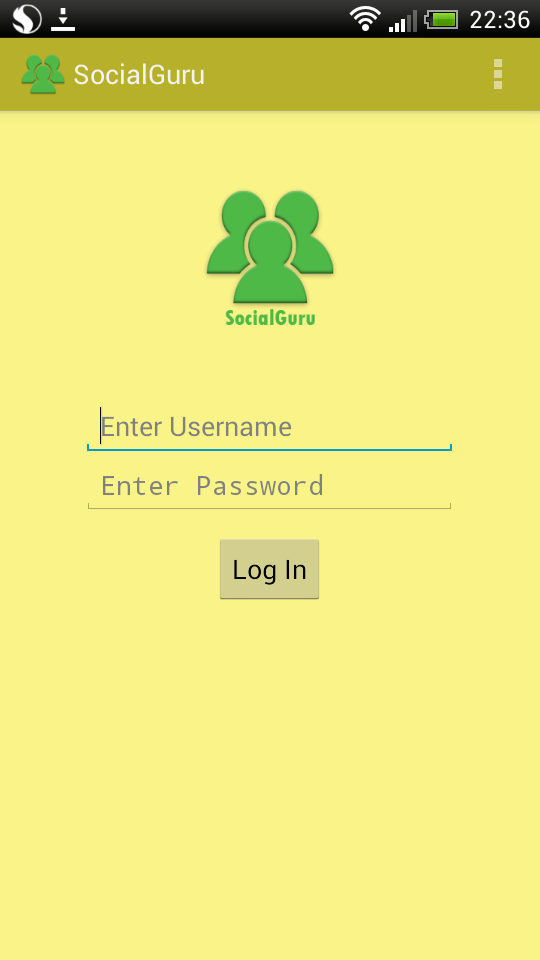
\includegraphics[scale=0.3]{images/nolibrary.png}
\caption{Application with only conventional method.}
\label{fig:nolibrary}
\end{figure}

\begin{figure}[H]
\begin{center}
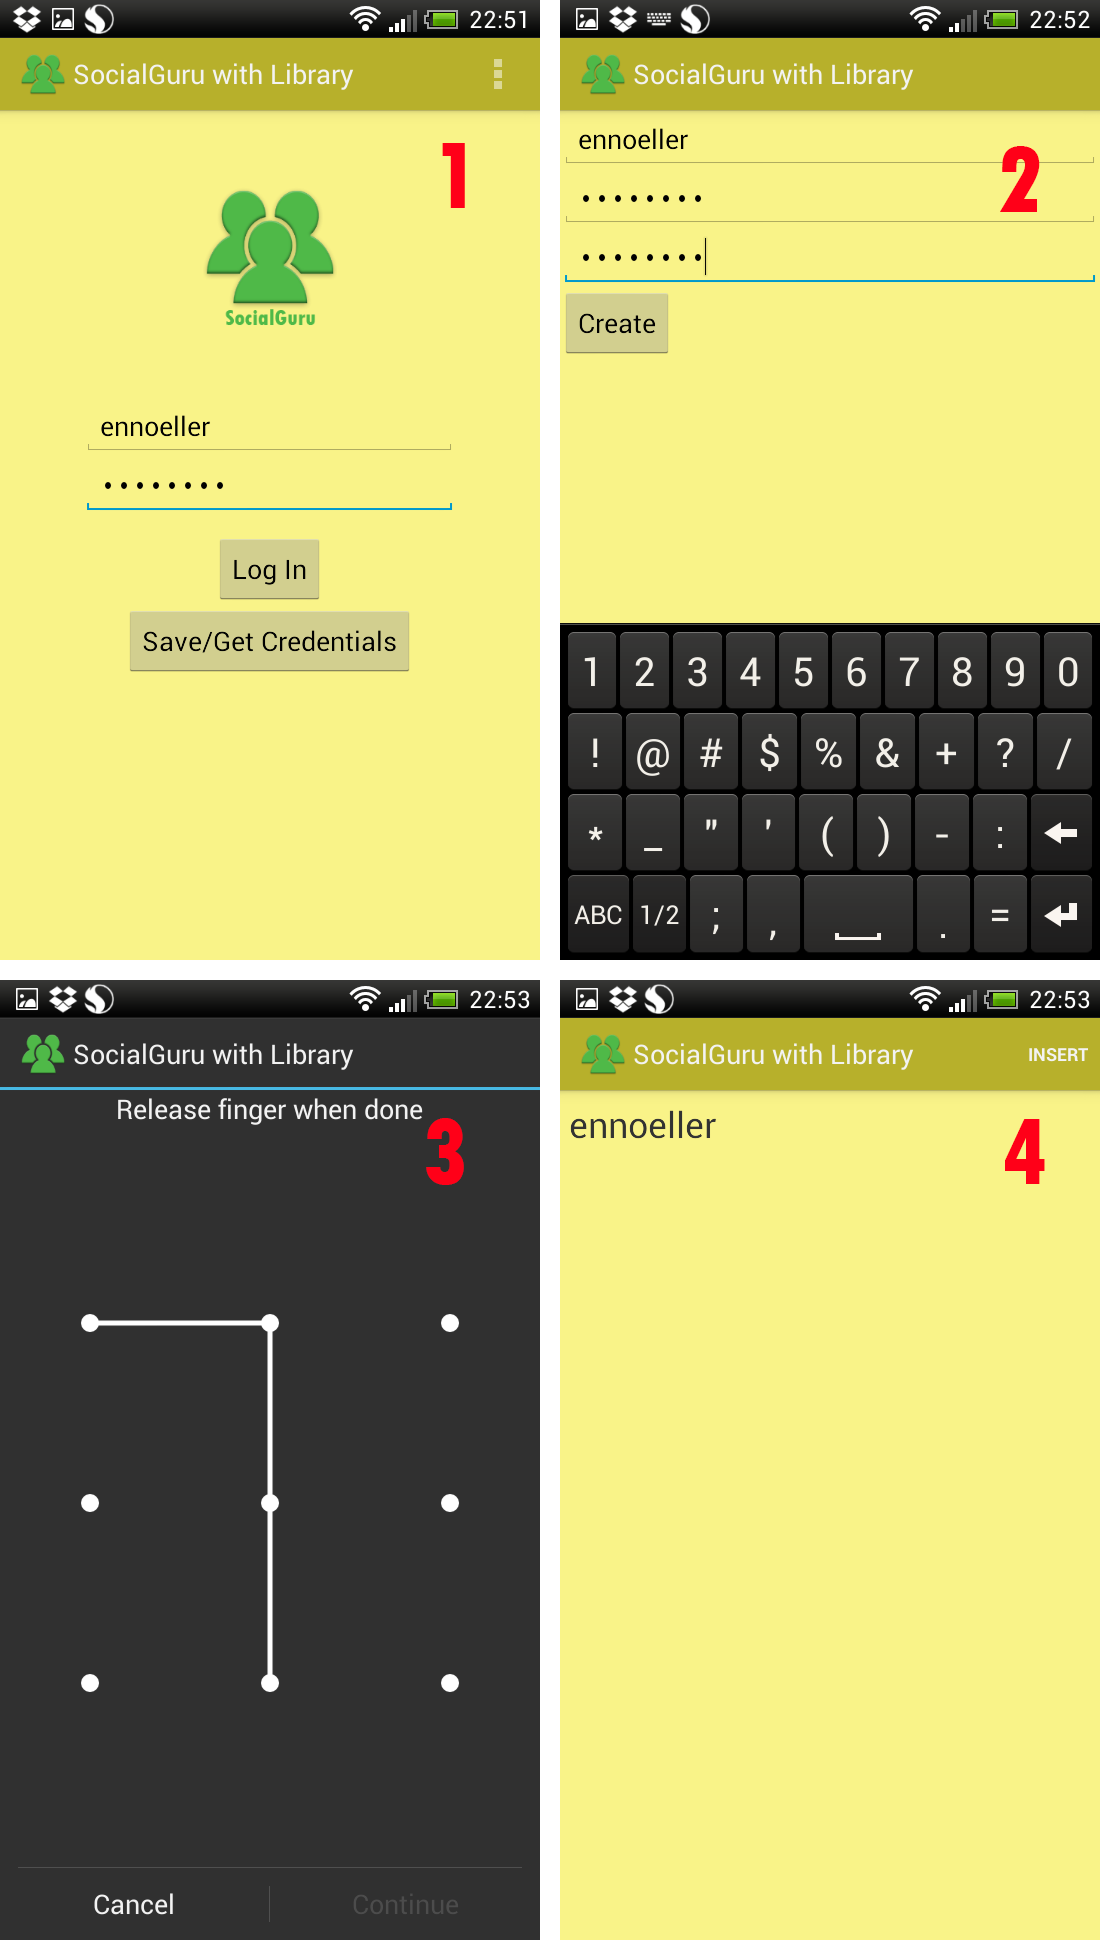
\includegraphics[scale=0.3]{images/reg.png}
\caption{Credentials saving process with the library.}
\label{fig:credentials saving}
\end{center}
\end{figure}

\begin{figure}[H]
\begin{center}
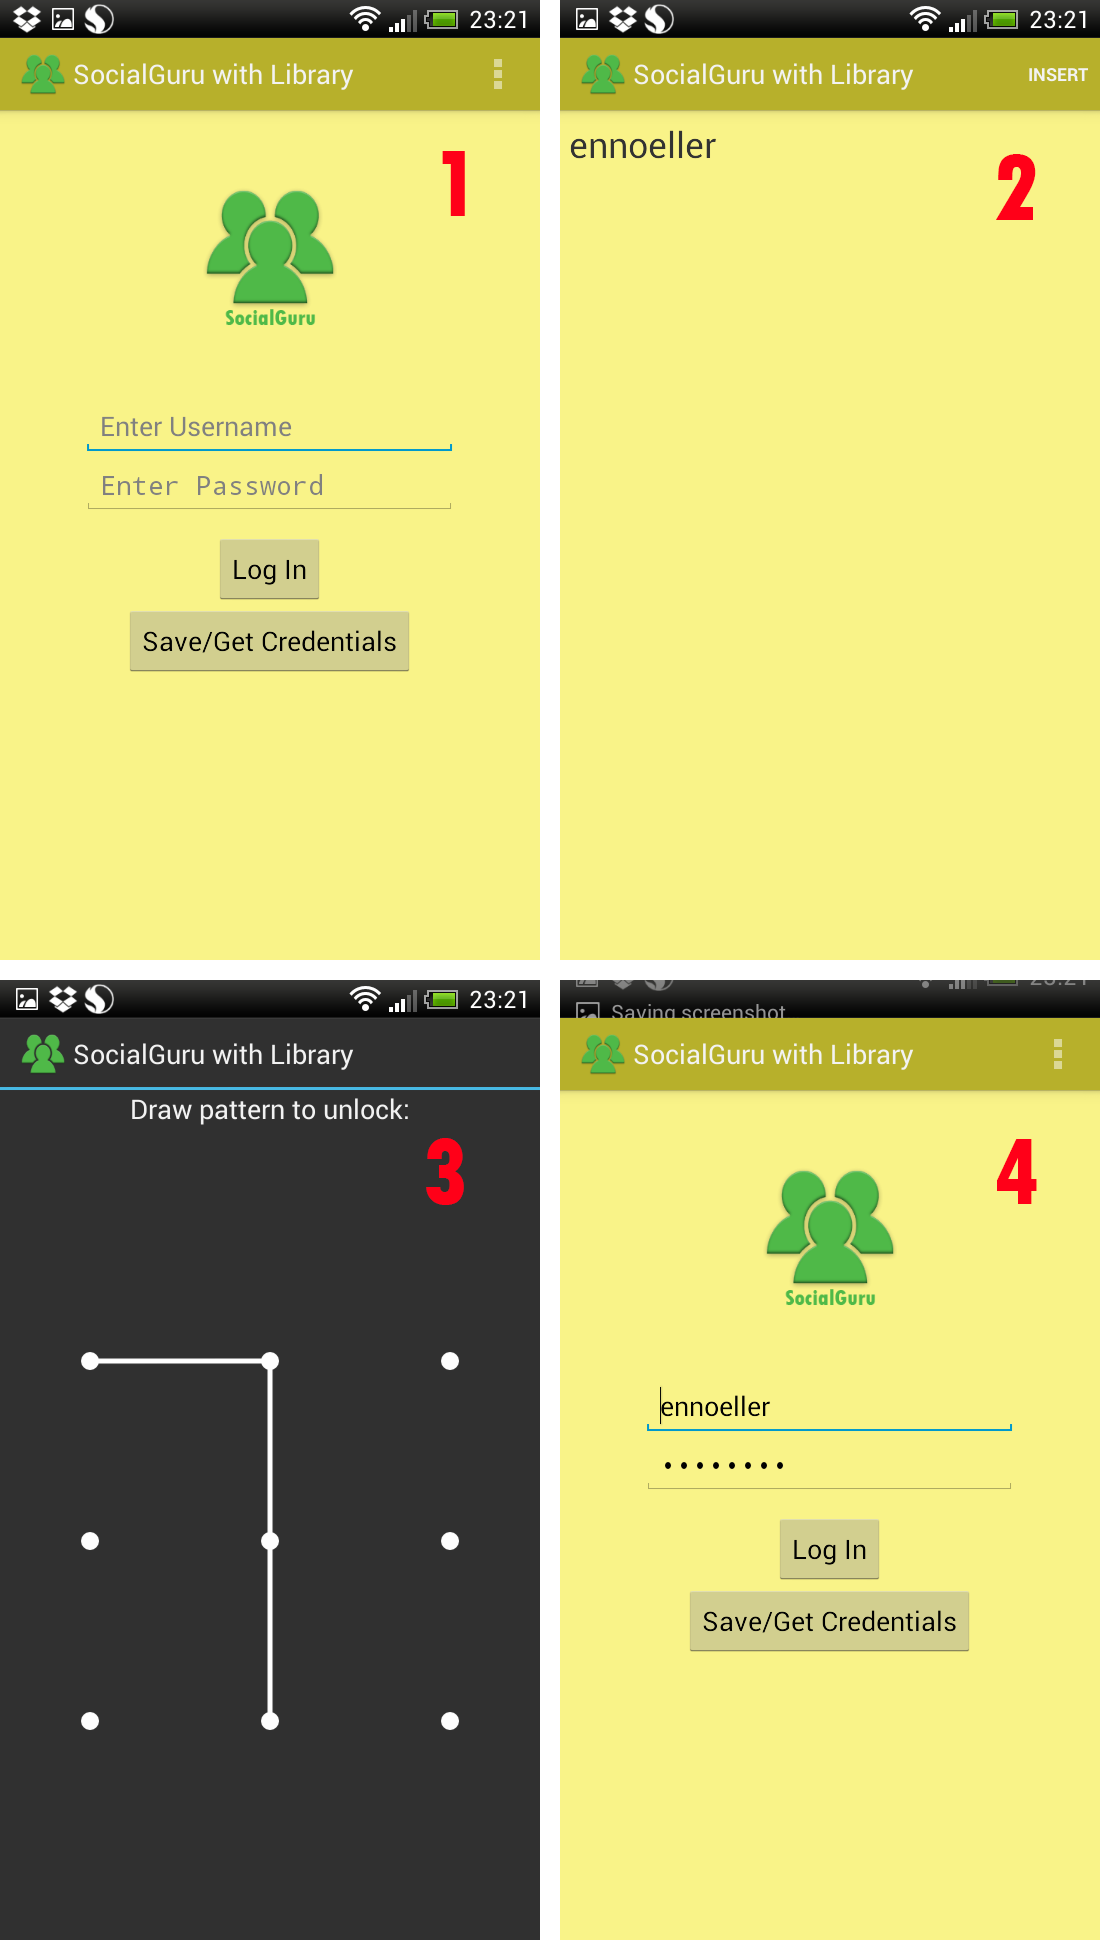
\includegraphics[scale=0.3]{images/auth.png}
\caption{Athentication process with the library.}
\label{fig:authentication}
\end{center}
\end{figure}

\section{Results}

First two questions were about participants opinions about authentication methods used in applications. 65\% of them, shown in Figure 5.4, find that applications do use suitable login methods. 5 out of 7 participants, who find applications not to use suitable methods, brought out that the process should include less typing. 

\begin{figure}[H]
\centering
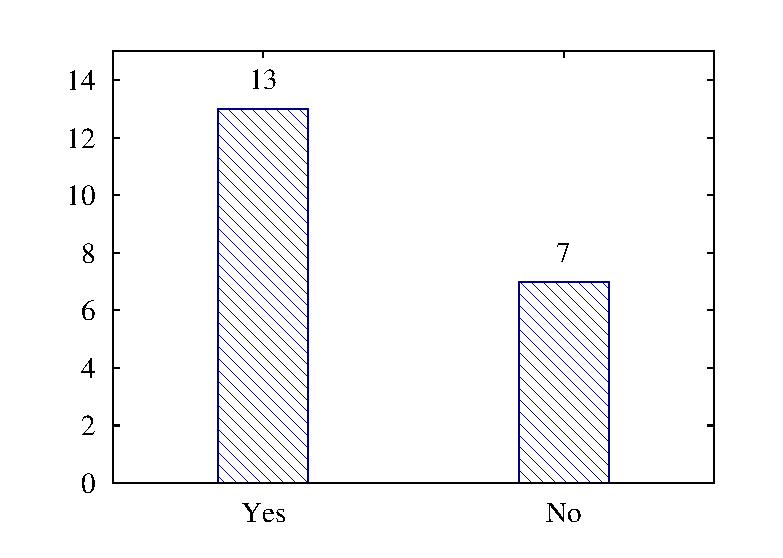
\includegraphics[scale=.7]{files/question1/question1.eps}
\caption{Do apps use suitable login methods?}
\label{fig:digraph}
\end{figure}

\subsection{Participants Opinion on Conventional Login}
Most of the participants found the authentication method to be normal or even hard for them as seem on the Figure 5.5, implying to the size of the keyboard on the device. The same \% applied to the question, if they were annoyed by the process, shown at Figure 5.6. Given the answers values of 1 to 3, 1 being ''Easy/Low'', the average to both of these questing would be 2.15. 

As seen from the Figures 5.7 and 5.8, the conventional login method would push users away from the application or make them change their passwords to something easier to type. Seven participants would definitely use the application less and six are considering it, making the applicatio less appealing to 65\% of users because of the authentication process. This method is also pushing 70\% of the  users to change their passwords, making them more vulnerable to intruders.  

This shows how damaging the conventional method could be for the user base and reputation of the application. Also users are put to danger by allowing themselves to use weaker passwords.

\begin{figure}[H]
\centering
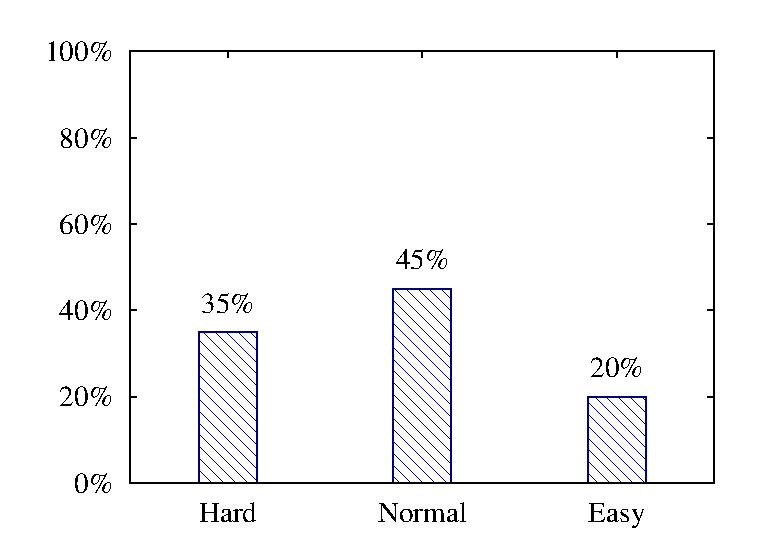
\includegraphics[scale=.7]{files/question3/question3.eps}
\caption{Difficulty to authenticate using apps that require login credentials?}
\label{fig:digraph}
\end{figure}

\begin{figure}[H]
\centering
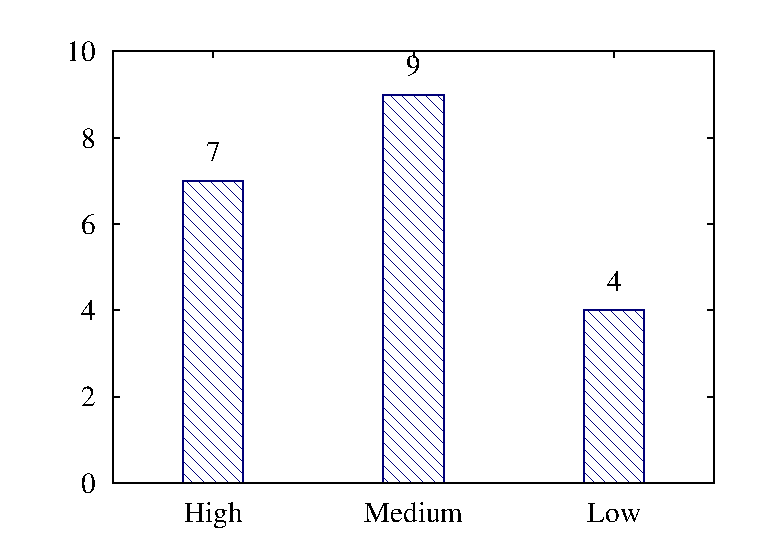
\includegraphics[scale=.7]{files/question4/question4.eps}
\caption{How annoying would you rate the login process in a mobile app?}
\label{fig:digraph}
\end{figure}

\begin{figure}[H]
\centering
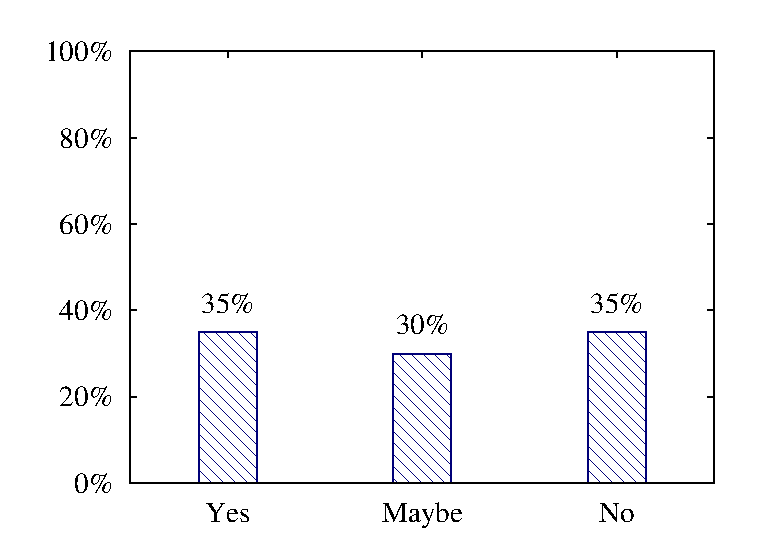
\includegraphics[scale=.7]{files/question5/question5.eps}
\caption{If the application required login every week, would you use it less because of the inconvenience?}
\label{fig:digraph}
\end{figure}

\begin{figure}[H]
\centering
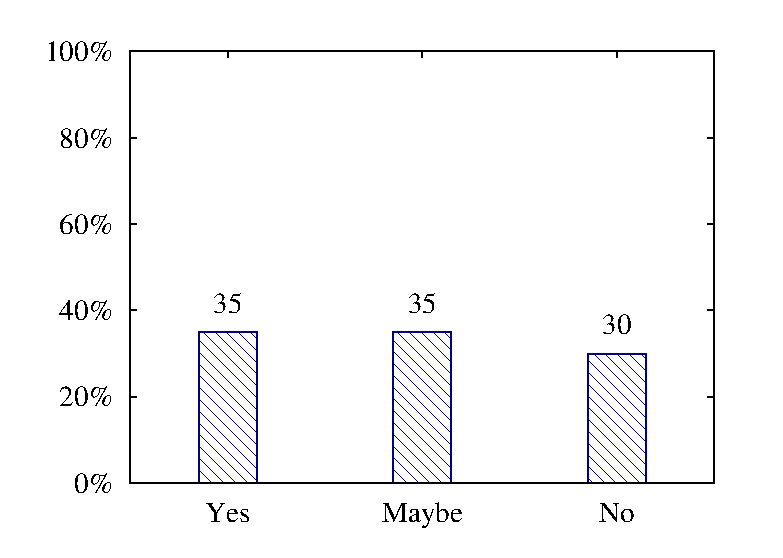
\includegraphics[scale=.7]{files/question6/question6.eps}
\caption{If the application required login every week, would you change your password to something easier to type (weaker)?}
\label{fig:digraph}
\end{figure}

\subsection{Participants Opinion on the Proposed Solution}

The participants were using this method for the first time and were asked questions about the simplicity of it, to see whether this solution could be justified. 

Compared to the conventional method, the proposed solution seems to be easier to use for the participants, see the Figure 5.9. Nobody thought it was hard. 75\% of the participants found the method easy and 25\% normal. Given the answers values of 1 to 3, 1 being ''Easy'', the average would be 1.25. This is also reflected on usage of the application, where nobody answered they would use the application less, shown on Figure 5.10, because of the provided method. Only 15\% of participants would consider using it less. 

The given method was composed of two steps. Before authenticating themselves, they had to register their credentials with the application. 75\% of the participants found the process easy and nobody felt confused, as seen on Figure 5.11. When asked to change the password or pattern saved in the application, some participants felt confused in the process - 25\%, but 55\% found it intuitive, as seen in Figure 5.12.

\begin{figure}[H]
\centering
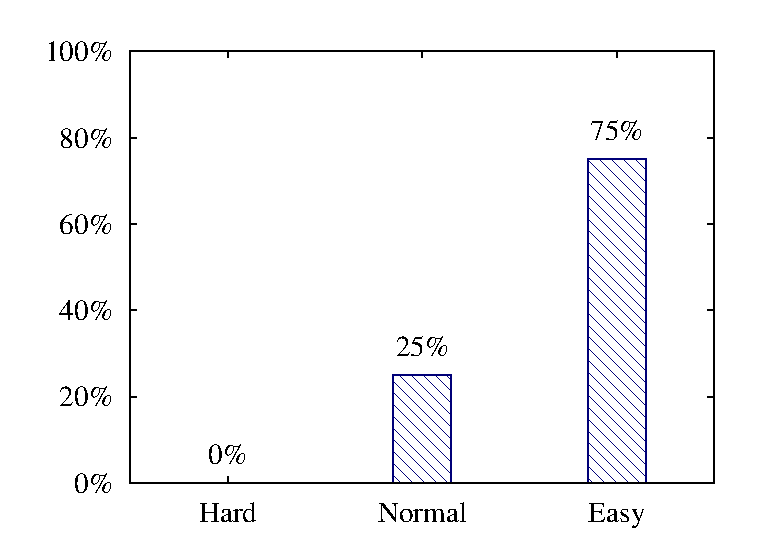
\includegraphics[scale=.7]{files/question7/question7.eps}
\caption{Difficulty to authenticate using the pattern-based method?}
\label{fig:digraph}
\end{figure}

\begin{figure}[H]
\centering
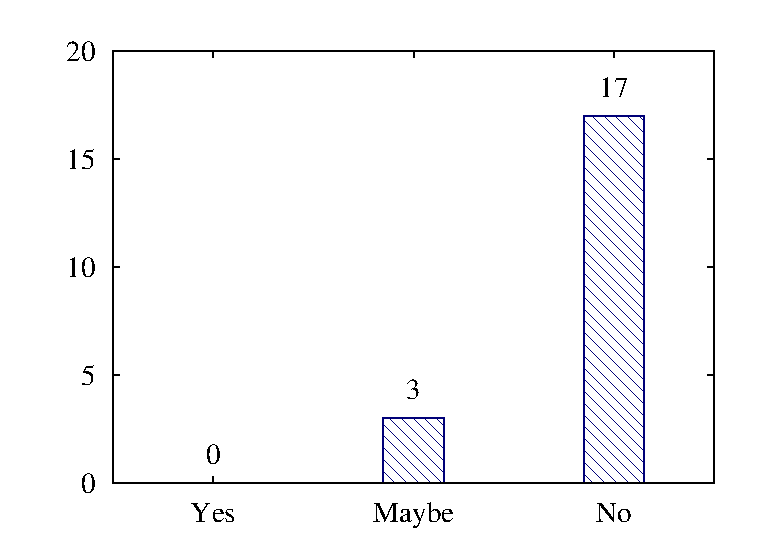
\includegraphics[scale=.7]{files/question8/question8.eps}
\caption{If the application required login every week, would you use it less because of the inconvenience?}
\label{fig:digraph}
\end{figure}

\begin{figure}[H]
\centering
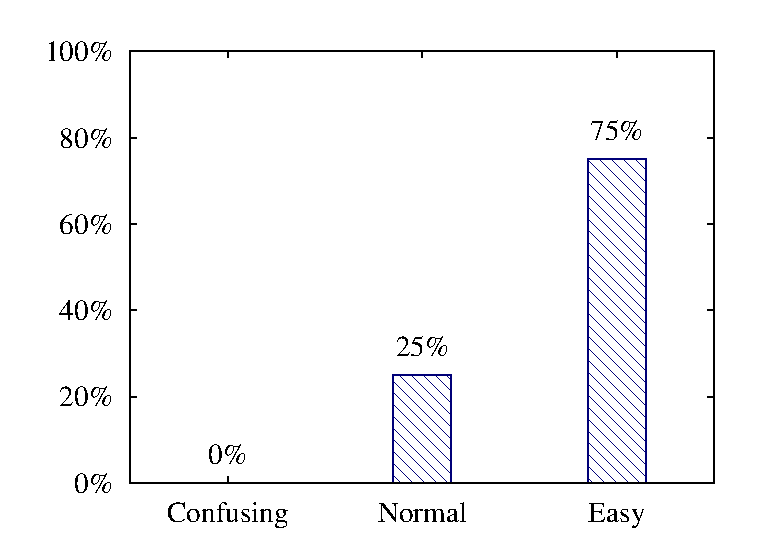
\includegraphics[scale=.7]{files/question9/question9.eps}
\caption{How intuitive was the process of saving your authentication credentials?}
\label{fig:digraph}
\end{figure}

\begin{figure}[H]
\centering
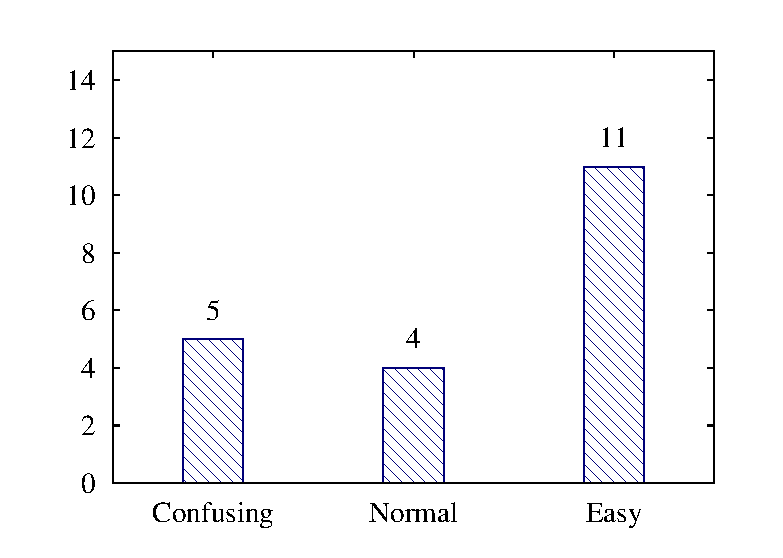
\includegraphics[scale=.7]{files/question10/question10.eps}
\caption{How intuitive was the process of editing the password or pattern?}
\label{fig:digraph}
\end{figure}

\section{Summary}
In this chapter the usability of the proposed mechanism is validated.  With the conventional model, 35\% of the participants found it hard and annoying. It was also pushing people away from the product or making them change their passwords to something less secure. Opposed to the conventional method, the proposed solution was easier to the user, as 75\% of the participants found it easy to use and therefore they were not losing interest in the application. Though some participants were confused in changing password or pattern, the process itself should be clear once it has been done for the first time. 

Although the group of participants was only 20 people of a 10 year age gap, the results strongly indicate the feasibility of this solution.



% ---------------------------------------------------------------------------
%: ----------------------- end of thesis sub-document ------------------------
% ---------------------------------------------------------------------------

